\subsection{Effects of Different Hyperparameters}
\label{sec:subtask3}

In this task, we study the effects of hyperparameters such as the optimizer, learning rate, weight decay, dropout and batch size.
For all experiments in this section, we set $p = 97$ and use the transformer model.
Our baseline setting has the same hyperparameters as mentioned at the beginning of \cref{sec:subtask1}.
% The results are shown in \cref{fig:different_settings}.
% Similarly, the training accuracies raise up to $99\%$ within $10^3$ steps in most experiments, but the validation accuracies differ from each other.

\begin{figure}[!ht]
    \centering
    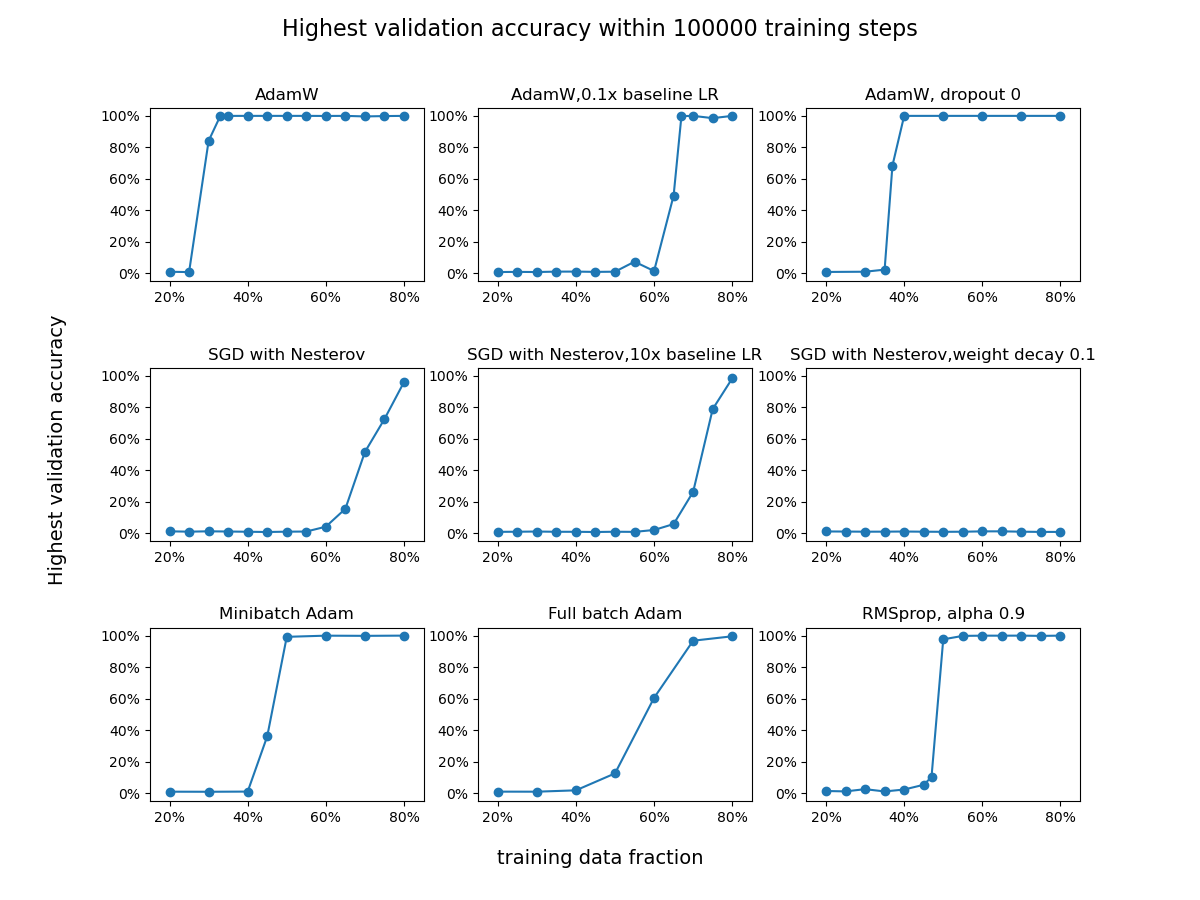
\includegraphics[width=0.9\textwidth]{fig/different_settings/different_settings.png}
    \caption{Grokking phenomenon for different settings.
    Top left: Baseline setting (see \cref{sec:subtask1}).
    Top center: Baseline setting with learning rate $10^{-4}$.
    Top right: Baseline setting with dropout $0$.
    Middle left: SGD with Nesterov, weight decay $0$, learning rate $10^{-3}$.
    Center: SGD with Nesterov, weight decay $0$, learning rate $10^{-2}$.
    Middle right: SGD with Nesterov, weight decay $0.1$, learning rate $10^{-3}$.
    Bottom left: Mini batch Adam with weight decay $0$.
    Bottom center: Full batch Adam with weight decay $0$.
    Bottom right: RMSprop with $\alpha = 0.9$, weight decay $0$.
    }
    \label{fig:different_settings}
\end{figure}
\begin{figure}[!ht]
    \centering
    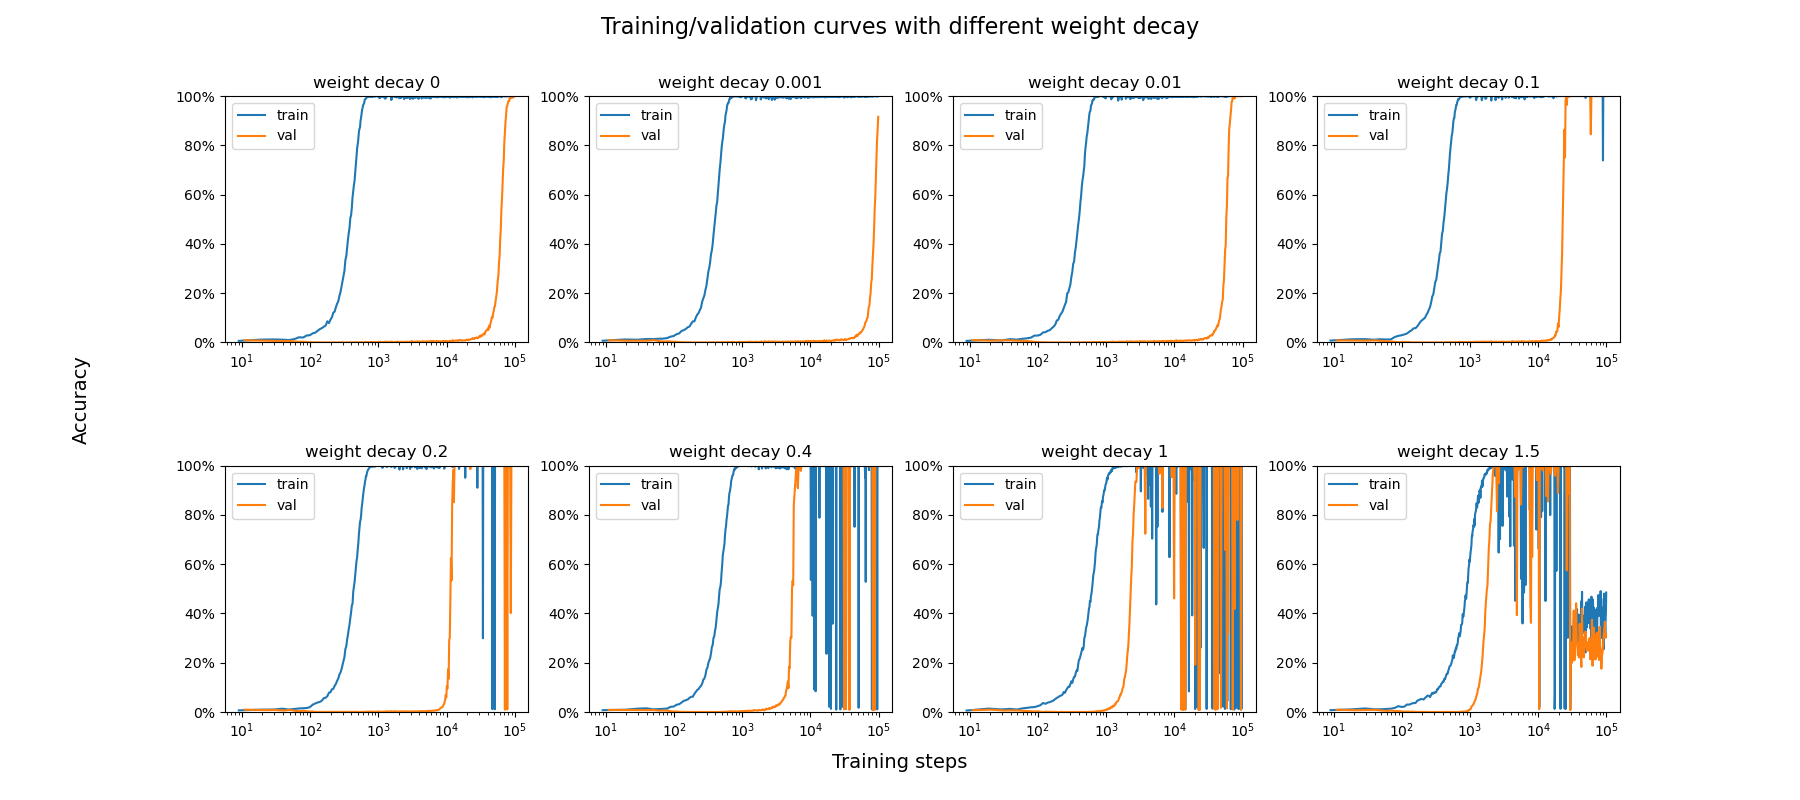
\includegraphics[width=0.9\textwidth]{fig/weight_decay/weight_decay.png}
    \caption{Grokking phenomenon for different weight decay}
    \label{fig:different weight_decay}
\end{figure}

It can be seen from \cref{fig:different_settings} that the model generalizes well in the baseline setting for training data fraction $\alpha = 33\%$, but does not generalize even for $\alpha = 60\%$ when the learning rate is changed into $10^{-4}$.
This is because a small learning rate slows down training.
However, big learning rates do not necessarily speed up training, which can be seen by comparing the first two figures on the second row. 
Removing dropout has little impact on AdamW (top right).
Adding weight decay makes SGD's training even worse (middle right).
As for the comparison between optimizers, under the same learning rate and dropout settings, AdamW is the best and SGD with Nesterov acceleration is the worst.
RMSprop and mini batch Adam have acceptable performance when $\alpha \geq 50\%$, while full batch Adam needs to exceed $70\%$ to reach the same level.

We further study the impact of weight decay by training the transformer model with AdamW optimizer with different weight decay.
The results are plotted in \cref{fig:different weight_decay}.
As the weight decay increases, the generalization becomes easier, and the grokking phenomenon becomes less obvious. 
However, it is worth noting that when the weight decay exceeds $0.2$, there are occasional ``rollback'' phenomena in training accuracy and validation accuracy on certain training steps, which occur more frequently as the weight decay increases. 
When the weight decay is $1.5$ and the number of training steps exceeds $3 \times 10^4$, accuracy cannot even be restored. 
The reason is worth further exploration, but at least it tells us that the selection of training steps does not need to be too large.